\documentclass[a4paper,12pt]{article}
%%%%%%%%%%%%%%%%%%%%%%%%%%%%%%%%%%%%%%%%%%%%%%%%%%%%%%%%%%%%%%%%%%%%%%%%%%%%%%%%%%%%%%%%%%%%%%%%%%%%%%%%%%%%%%%%%%%%%%%%%%%%%%%%%%%%%%%%%%%%%%%%%%%%%%%%%%%%%%%%%%%%%%%%%%%%%%%%%%%%%%%%%%%%%%%%%%%%%%%%%%%%%%%%%%%%%%%%%%%%%%%%%%%%%%%%%%%%%%%%%%%%%%%%%%%%
\usepackage{eurosym}
\usepackage{vmargin}
\usepackage{amsmath}
\usepackage{graphics}
\usepackage{epsfig}
\usepackage{enumerate}
\usepackage{multicol}
\usepackage{subfigure}
\usepackage{fancyhdr}
\usepackage{listings}
\usepackage{framed}
\usepackage{graphicx}
\usepackage{amsmath}
\usepackage{chngpage}
%\usepackage{bigints}

\usepackage{vmargin}
% left top textwidth textheight headheight
% headsep footheight footskip
\setmargins{2.0cm}{2.5cm}{16 cm}{22cm}{0.5cm}{0cm}{1cm}{1cm}
\renewcommand{\baselinestretch}{1.3}

\setcounter{MaxMatrixCols}{10}

\begin{document}
\large 
\noindent A statistician is carrying out an exercise to analyse a dataset that describes the failure
times of outdoor telephone cables, with respect to the cable material quality (graded
1 to 4) and level of rainfall in centimetres that the cable is exposed to.

\medskip
\noindent The data given in the file “\texttt{CablesDataset.csv}” show failure times in years for 20
different cables.



\begin{framed}\begin{verbatim}
# read the data
cables_data<-read.csv("CablesDataset.csv")
head(cables_data)
\end{verbatim} \end{framed}

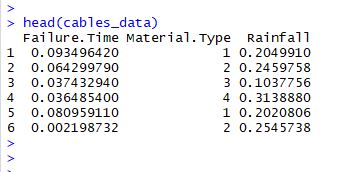
\includegraphics[scale=1.5]{00-A1/images/CablesData_1_head.JPG}

\newpage 

%%%%%%%%%%%%%%%%%%%%%%%%%%%%%%%%%%%%%%%%%%%%
\subsection*{Exercise 1}
\noindent  Fit a linear model to the data with the failure time as the response, including
both cable material quality and level of rainfall as the two covariates. Your
answer should include a summary of the fitted model.\\
\medskip 




\begin{framed}\begin{verbatim}
# fit the linear model

linear_model<-lm(Failure.Time~Material.Type + Rainfall,
cables_data)

# output the linear model fit summary statistics
summary(linear_model)
\end{verbatim} \end{framed}

\newpage 
\begin{verbatim}
   Call:
    lm(formula = Failure.Time ~ Material.Type +
        Rainfall, data = cables_data)
    
    Residuals:
          Min        1Q    Median        3Q       Max 
    -0.051313 -0.006694  0.002246  0.008590  0.025763 
    
    Coefficients:
                   Estimate Std. Error t value Pr(>|t|)    
    (Intercept)    0.081086   0.012659   6.406 6.52e-06 ***
    Material.Type -0.014499   0.003575  -4.055 0.000822 ***
    Rainfall       0.005591   0.046745   0.120 0.906200    
    ---
    Signif. codes:  0 ‘***’ 0.001 ‘**’ 0.01 ‘*’ 0.05 ‘.’ 0.1 ‘ ’ 1
    
    Residual standard error: 0.01627 on 17 degrees of freedom
    Multiple R-squared:  0.5326,	Adjusted R-squared:  0.4776 
    F-statistic: 9.687 on 2 and 17 DF,  p-value: 0.001556
    
\end{verbatim}    
 

\newpage 
%%%%%%%%%%%%%%%%%%%%%%%%%%%%%%%%%%%%%%%%%%%%
\subsection*{Exercise 2}

State the formula of the model fitted in Exercise 1, clearly explaining the
notation that you use.
Comment on the significance of the parameters of the model fitted.


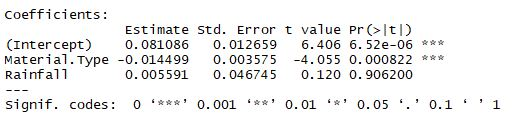
\includegraphics[scale=1.3]{00-A1/images/CablesData_2_modelsummary.JPG}


\noindent
\begin{itemize}
    \item From analysing the R output, we see that the fitted linear model is:
\[ \hat{y} = 0.081086 \;-;\ 0.014499x_1 \;+\; 0.005591x_2\]

where $x_1$ is the ‘material type’ variable, and $x_2$ is the ‘rainfall’ variable. $\hat{y}$ is the predicted failure time.


\item The R output shows that the ‘material type’ parameter is significantly
different to zero (at the 0.1\% level).
\item The ‘rainfall’ parameter is not significantly different to zero - this is
indicated by the t-tests shown in the fourth column of the R output.
\item The intercept is also significantly different to zero
\end{itemize}


\newpage 
%%%%%%%%%%%%%%%%%%%%%%%%%%%%%%%%%%%%%
\subsection*{Exercise 3}

\noindent Plot the residuals of the model. Comment on the plot.






\begin{framed}\begin{verbatim}
# obtain the residuals

residuals(linear_model)

\end{verbatim} \end{framed}


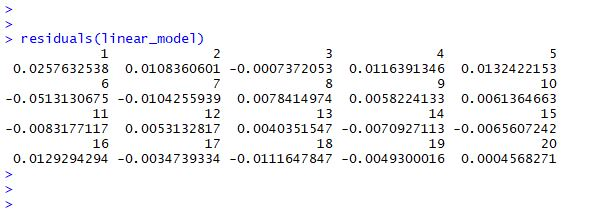
\includegraphics[scale=1.1]{00-A1/images/CablesData_3_residuals.JPG}


\newpage 

\begin{framed}\begin{verbatim}
# plot the residuals

plot(residuals(linear_model),
      pch=16,col="red",cex=1.4)

abline(h=0)

\end{verbatim} \end{framed}


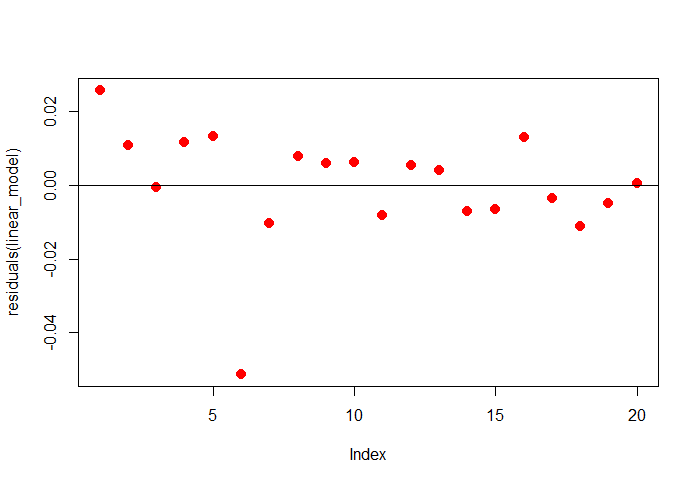
\includegraphics[scale=0.8]{00-A1/images/CableData_4_Residuals.png}



\noindent The residuals exhibit a fairly random scatter around zero
apart from the 6th point.


%%%%%%%%%%%%%%%%%%%%%%%%%%%%%%%%%%
\newpage 
\subsection*{Exercise 4}

\noindent An analyst suggests that the 6th row of the original data should be removed. Construct a new data set from the original data \textbf{\textit{CablesDataset.csv}}
with the 6th row removed. Justify the removal of the 6th row from the original data.


\begin{framed} \begin{verbatim}
# remove data point 6 and redefine the dataset

cables_data2 <- cables_data[-6,]
\end{verbatim} \end{framed}


\noindent The residuals plot indicates that data point 6 is an outlier.
%%%%%%%%%%%%%%%%%%%%%%%%%%%%%%%%%%%%%%%%%%55
\newpage 
\subsection*{Exercise 5}

\noindent Fit a linear model to the new data set constructed in Exercise 4. Comment on the fit of the new model compared to the model fitted previously, by comparing suitable statistics from the R
outputs.

\begin{framed}\begin{verbatim}
# refit the linear model

linear_model2 <- lm(Failure.Time~Material.Type + Rainfall,
    data = cables_data2)

summary(linear_model2)
\end{verbatim} \end{framed}

\newpage 
\begin{verbatim}
 
    Call:
    lm(formula = Failure.Time ~ Material.Type + Rainfall, 
        data = cables_data2)
    
    Residuals:
           Min         1Q     Median         3Q        Max 
    -0.0144060 -0.0082529 -0.0003768  0.0071557  0.0213878 
    
    Coefficients:
                   Estimate Std. Error t value Pr(>|t|)    
    (Intercept)    0.086629   0.008094  10.703 1.06e-08 ***
    Material.Type -0.015576   0.002275  -6.846 3.93e-06 ***
    Rainfall       0.005152   0.029621   0.174    0.864    
    ---
    Signif. codes:  0 ‘***’ 0.001 ‘**’ 0.01 ‘*’ 0.05 ‘.’ 0.1 ‘ ’ 1
    
    Residual standard error: 0.01031 on 16 degrees of freedom
    Multiple R-squared:  0.7756,	Adjusted R-squared:  0.7475 
    F-statistic: 27.64 on 2 and 16 DF,  p-value: 6.438e-06
\end{verbatim}

\begin{itemize}
    \item The adjusted $R^2$ statistic for the model fitted to the data with the outlier
removed is 0.7475. 
\item This shows an improved fit relative to the model fitted to all
20 data points, which had an adjusted $R^2$ statistic of 0.4776.
\end{itemize}


%%%%%%%%%%%%%%%%%%%%%%%%%%%%%%%%%%%%%%%%%%%

\newpage 
\subsection*{Exercise 6}
\noindent Fit a generalised linear model (GLM) to the data set constructed in
Exercise 4 using a Gamma distribution.
State the formula of the model fitted, clearly explaining
the notation that you use.
Comment on the significance of the parameters of the fitted model.


\begin{framed}\begin{verbatim}
# fit a Gamma GLM
gfit<-glm(Failure.Time~Material.Type+Rainfall,
        famil y= Gamma(link=inverse), 
        data = cables_data2)
\end{verbatim} \end{framed}

\newpage
\begin{verbatim}

Call:
glm(formula = Failure.Time ~ Material.Type + Rainfall,
    family = Gamma(link = inverse), 
    data = cables_data2)

Deviance Residuals: 
     Min        1Q    Median        3Q       Max  
-0.26231  -0.14156  -0.03338   0.12850   0.25185  

Coefficients:
              Estimate Std. Error t value Pr(>|t|)    
(Intercept)     6.1921     2.6184   2.365    0.031 *  
Material.Type   6.7286     0.8359   8.050 5.12e-07 ***
Rainfall        0.4814    10.6244   0.045    0.964    
---
Signif. codes:  0 ‘***’ 0.001 ‘**’ 0.01 ‘*’ 0.05 ‘.’ 0.1 ‘ ’ 1

(Dispersion parameter for Gamma family taken to be 0.03085425)

    Null deviance: 2.99847  on 18  degrees of freedom
Residual deviance: 0.48503  on 16  degrees of freedom
AIC: -125.54

Number of Fisher Scoring iterations: 4

\end{verbatim}
\newpage 


\begin{framed}\begin{verbatim}
coef(gfit)
\end{verbatim} \end{framed}


\begin{verbatim}
> coef(gfit)
  (Intercept) Material.Type      Rainfall 
    6.1920558     6.7286452     0.4814427 
> 
\end{verbatim}



\[
\hat{\eta} = \frac{1}{\mu} 
= 6.1920558 + 6.7286452x_1 + 0.4814427x_2
\]

where $x_1$ is the ‘material type’ variable, and $x_2$ is the ‘rainfall’ variable.

\newpage 

\begin{framed}\begin{verbatim}
# review the model fit
summary(gfit)
\end{verbatim} \end{framed}


 \begin{verbatim}
    Call:
    glm(formula = Failure.Time ~ Material.Type + Rainfall, 
        family = Gamma(link = inverse), 
        data = cables_data2)
 ...
    
    Coefficients:
                  Estimate Std. Error t value Pr(>|t|)    
    (Intercept)     6.1921     2.6184   2.365    0.031 *  
    Material.Type   6.7286     0.8359   8.050 5.12e-07 ***
    Rainfall        0.4814    10.6244   0.045    0.964    
    ---
    Signif. codes:  0 ‘***’ 0.001 ‘**’ 0.01 ‘*’ 0.05 ‘.’ 0.1 ‘ ’ 1
    
    (Dispersion parameter for Gamma family taken to be 0.03085425)
    
        Null deviance: 2.99847  on 18  degrees of freedom
    Residual deviance: 0.48503  on 16  degrees of freedom
    AIC: -125.54
    
    Number of Fisher Scoring iterations: 4
\end{verbatim}
%%%%%%%%%%%%%%%%%%%%%%%%%%%%%%%
\newpage
Reviewing the model fit output from R, the ‘rainfall’ parameter is not
significantly different to zero, whereas the ‘material type’ parameter is
significant at the 0.1\% level.
\end{document}